\section{Methodology}
Similarly to 
\cite{krauss2016arbitrageSandP} 
and \cite{krauss2019statisticalArbitrage},
the methodology of this paper consists of
the following steps:

\begin{enumerate}
    \item The entire data set is split into a training, a validation and a trading set.
    \item The respective features (explanatory variables) and targets (dependent variables) are created
    \item Each model is trained on the training set
    \item Conduct out-of-sample predictions on the trading set for each model 
    \item Evaluate its accuracy and trading-performance on the trading set respectively
    \item Go to Step 2, and repeat the same steps for a different feature- and target-specification
\end{enumerate}



%%% TRAINING AND TRADING SET
\subsection{Training and Trading Set} \label{ch:training_trading}
In our application to minute-binned data, the test set, i.e. trading set, contains all observations from 01.11.2019 to 31.12.2019.
The training set ranges from 01.01.2019 to 14.09.2019, and the remaining 15.09.2019 to 31.10.2019 
is reserved for the valdation set. We decided against the usual k-fold cross-validation approach 
in order to emphasize the importance of future observation for the model, since its performance only gets
evaluated on the future trading set. The daily cumulative short returns in the trading period of the top ten coins can
seen below in figure \ref{fig:all_top_10_daily_cum_returns}. The returns in the trading period 
exhibit a downward trajectory across all coins, thus the positive short returns.

\begin{figure}[H] 
    \captionsetup{format=plain}
    \makebox[\textwidth]{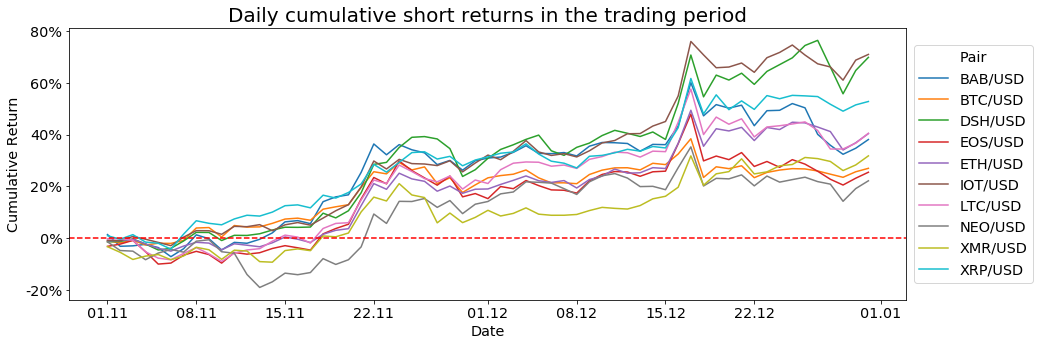
\includegraphics[width=160mm]{all/all_top_10_daily_cum_returns.png}}
    \caption{
        This figure illustrates daily cumulative short returns in the trading period for the top ten coins selection.
    }
    \label{fig:all_top_10_daily_cum_returns}
\end{figure}


%%% FEATURE AND TARGET GENERATION
\subsection{Feature and Target Generation} \label{ch:feature_and_target}
Broadly following \cite{takeuchi2013momentumTrading},
we generate the feature space as follows:

Let $ P^{c} = ( P^{c}_{t} )_{t \in T} $ denote the price process of coin-USD-pair $ c $, with $ c \in \{1, ... , n\} $. The price itself is the average between \textit{Open} and \textit{Close}.

\begin{description}
    \item[Features:] From the data set we obtain the following features:
    \begin{description}
        \item[Returns:] Let $ R^{c}_{t, t - m} $ be the simple return for coin $ c $ over $ m $ periods defined as
        \begin{equation}
            \label{eq:return}
            R^{c}_{t, t - m} = \frac{ P^{c}_{t} }{ P^{c}_{t - m} } - 1 
        \end{equation} 
        \item[Volumes:] {
            Let $ V^{c}_{t} $ be the traded volume for coin $ c $ in minute-bin $ t $ scaled by Quantile-Transformer 
            fitted separately for each coin only on bins with $ V^{c}_{t} > 0 $. 
        }
    \end{description}
    \item[Target:] {
        Let $ Y^{c}_{t + d, t} $ be a binary response variable for each coin $c$ 
        and $ d = 120, 240 $ the size of the future time interval. 
        It assumes value 1 (class \textit{up}) if its future $d$ min return $ R^{c}_{t + d + 1, t + 1} $ is greater 
        than its cross-sectional median across all pairs $ ( R^{c}_{t + d + 1, t + 1} )^{C}_{c=1} $, 
        else -1 (class \textit{down}). 
        Instead of just using the simple return $ R^{c}_{t + d + 1, t + 1} $ as in \cite{krauss2019statisticalArbitrage},
        we included an additional condition, which demands that $  V^{c}_{t + d + 1} > 0 $ for realizing the feature return.
        If not skip bins until you reach a bin $ t^{*} = t + d + \delta $  in which $  V^{c}_{ t^{*} } > 0 $, 
        then realize return as in equation \ref{eq:return}.
    }
\end{description}


The reason for this further restriction is to make the training of the model more similar to the 
trading decisions in the backtest, since we only allow trades to be executed in a bin, 
if any volume was traded for the respective coin.
We decided for the inclusion of volume such that the model has a measure for 
taking trading activity into account without breaking vital assumptions needed for testing 
the 1. Efficient Market Hypothesis (\cite{malkiel2003marketHypothesis}, \cite{fama1970marketHypothesis}).
In addition, the volume got scaled for each coin in order to make the measure more comparable across coins,
since we are training a single universal model for each of the selected coins. 
Further, the Quantile-Transformation handles outliers (<cite>) and restricts the feature to an intervall ranging from 0 to 1.

Let $ \tau $ denote the transaction cost per trade in basis points (bps) proportional to the traded amount.
For sake of simplicity, assume that we denote diffenrentiate between maker and taker transaction costs,
thus having equal transaction cost $ \tau = \tau_{taker} = \tau_{maker} $.
Incorporating costs $\tau$ leads to following expression for return $ R_{t, t-m}^{c} $ in long position,

\begin{equation} \label{eq:return_transaction_cost_long}
\begin{aligned}
    R_{t, t-m}^{c, long} &= \frac{ P_{t}^{c}(1 - \tau) - P_{t - m}^{c}(1 + \tau) }{ P_{t - m}^{c}(1 + \tau) }\\
    &= \frac{ P_{t}^{c} }{ P_{t - m}^{c} } \frac{ 1 - \tau }{ 1 + \tau } - 1,
\end{aligned}
\end{equation}

and analogously for the short position,

\begin{equation} \label{eq:return_transaction_cost_short}
    \begin{aligned}
        R_{t, t-m}^{c, short} = \frac{ P_{t - m}^{c} }{ P_{t}^{c} } \frac{ 1 - \tau }{ 1 + \tau } - 1
    \end{aligned}
\end{equation}

There


%%% MODEL TRAINING
\subsection{Model Training}
As explained in chapter \ref{ch:training_trading}, we construct a training set ranging 01.01.2019 to 14.09.2019, 
a validation set ranging from 15.09.2019 to 31.10.2019, and a trading set ranging from 01.11.2019 to 31.12.2019.
Further, we restrict the training and validation set by excluding bins for which no volume 
was traded in the following bin or lagged values are not available.


We cross-validate the respective parameter space by first training the model
on the test set an evaluating on the chronologically following validation set for each parameter combination.
After obtaining an accuracy evaluation of each combination, we fit the model with the best validation performance on
the combined training and valdation set.

Further, we also give a brief description of the models and how we used them for our trading experiments.
Before doing so, we introduce the mathematical notation. 
Let $ D = \{ (x_{i}, y_{i}) \}_{i=1}^{n} $ denote training data set containing $ n $ observations on which the respective model gets fitted
whereas $ x_{i} \in \mathbb{R}^{K} $ the denotes feature vector with $K$ features and $ y_{i} $ the target class variable for the $ i $-th observations respectively.
In addition, we denote a Decision Tree \cite{breiman1984decisionTree} as a function $ T_{D}^{q}(x) $ with $ D $ denoting the set which is was trained on,
$ q $ the selection of features it was trained on and $ x $ feature vector as an the function argument.
Decision Trees $ T_{D}^{q}(x) $ are used in Random Forest and AdaBoost.




\subsubsection{Logistic Regression} \label{ch:logistic_regression}
Logistic Regression sometimes called the logistic model or logit model,
analyzes the relationship between multiple independent variables or features and a
categorical dependent variable or target, and estimates the probability of occurrence
of an event by fitting data to a logistic curve. There are two models
of logistic regression, binary Logistic Regression and multinomial Logistic
Regression. Binary Logistic Regression is used in our application, since the dependent
variable is dichotomous ( either \emph{down}- or \emph{up}-movement, i.e. 0 or 1).

The building block for the Logistic Regression is the multiple regression model (\cite{james2013statisticalLearning}, \cite{park2013logisticRegression}),


\begin{equation}
    y = \sum_{j=1}^{J} \beta_{j} X_{j} + \epsilon =  X^{T}\beta + \epsilon
\end{equation}

with $y \in \mathbb{R}$ denoting the binary target, $\beta_{j}$ the parameter assigned to the $j$-th feature $X_{j}$ 
and $\epsilon$ the error term.
A problem that occurs when applying the multiple regression model is that the predicted values might
not fall between 0 and 1, thus not being eligible for estimating a probability $p(X)$.
Any time a straight line is fit to a binary response that is coded as
0 or 1, in principle we can always predict $p(X) < 0$ for some values of $X$
and $p(X) > 1$ for others (unless the range of X is limited) (<intro statistics>).
Therefore, to avoid this problem in the Logistic Regression, 
we wrap the \emph{logistic function} around the multiple regression model,

\begin{equation} \label{eq:logistic_function}
    p(X, \beta) = \frac{ \exp( X^{T}\beta ) }{ 1 + \exp( X^{T}\beta ) } = \frac{ 1 }{ 1 + \exp( -X^{T}\beta ) }
\end{equation}

Thus, the model can be written as,

\begin{equation}
    y = p(X, \beta) + \epsilon
\end{equation}


In order to estimate the coefficients $\beta$, we can use the \emph{maximum likelihood} method.
The basic intuition behind using maximum likelihood
to fit a logistic regression model is as follows: we seek estimates for $\beta$
such that the predicted probability $p(x_{i}, \beta)$ of the price movement for each observed feature vector $x_{i}$,
using equation \ref{eq:logistic_function},
corresponds as closely as possible to the observed price movement $y_{i}$.
This intuition can be formalized using a
mathematical equation called a \emph{likelihood function}:

\begin{equation}
    \mathscr{L}(\beta) = \prod_{i=1}^{n} p(x_{i}, \beta)^{y_{i}} (1 - p(x_{i}, \beta))^{1 - y_{i}}
\end{equation}

Therefore, we have the following optimization problem for the Logistic Regression:

\begin{equation}
    \beta^{*} = \argmax\limits_{ \beta \in \mathbb{R}^{J} } \mathscr{L}(\beta)
\end{equation}

We decided to use the Logistic Regression for predicting price movements, 
because it is relatively easy to interpret and it was used extensively 
as a benchmark in the related literatur (\cite{fischer2017lstmMarketPrediction}, \cite{krauss2019statisticalArbitrage}). 
For this paper, we rely on the Scikit-learn implementation of \cite{sklearn2011} for the logistic regression
and follow the parameters outlined in \cite{fischer2017lstmMarketPrediction}, i.e., the optimal L2-regularization is
determined among 100 values on a logarithmic scale from 0.0001 to 10,000 via cross-validation explained above
on the respective training set, and L-BFGS is deployed to find an optimum. 
Further, we restrict the maximum number of iterations to 100.


%%% RANDOM FOREST %%%
\subsubsection{Random Forest} \label{ch:random_forest}

Before outlining the algorithm for the Random Forest, we explain the essential 
building block of the Random Forest which is the Decision Tree.

The Decision Tree is a non-parametric supervised learning method used for classification and regression.
It predicts the response with a set of if-then-else decision rules derived from the data.
The deeper the tree, the more complex the decision rules and the closer the model fits the data.
The Decision Tree builds classification or regression models in form of a tree structure.
Each node in the tree further partions the feature space into smaller and smaller subsets, 
while at the same time an associated Decision Tree is incrementally developed.
The final result is a tree with decision nodes and terminal nodes. 
A decision node has two or more branches.
Leaf nodes represent the actual classification or decision. 
The topmost decision node in a tree which corresponds to the best predictor is called the root node.
Decision trees can handle both categorical and numerical data.

An example of such a tree is depicted below in figure \ref{fig:decision_tree_example}.

\begin{figure}[H]
    \captionsetup{format=plain}
    \makebox[\textwidth]{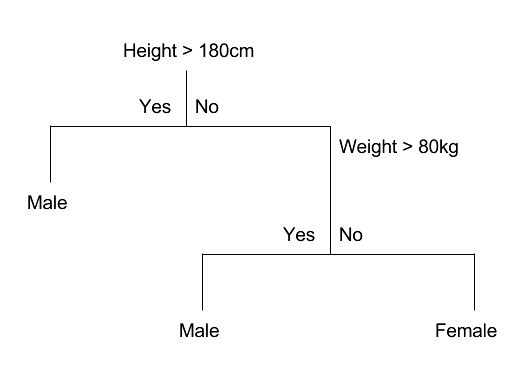
\includegraphics[width=100mm]{forest/decision_tree_example.png}}
    \caption{Given a data set with two features height and weight, and gender as the target variable, 
             this example tree stratisfies the two-dimensional feature space into three distinct subset each 
             represented by the terminal nodes at the bottom.
             The stratification occurs at the two deciding nodes depending either on whether its height is above 180 cm 
             and its weight is above 80kg.
             }
    \label{fig:decision_tree_example}
\end{figure}

In the following, we describe the CART algorithm for tree building as specified in \cite{breiman1984decisionTree}.
The basic idea of tree growing is to choose a split among all the possible splits at each node
such that the resulting child nodes are the "purest". In this algorithm, only univariate splits are
considered. That is, each split depends on the value of only one predictor variable. All
possible splits consist of possible splits of each predictor.

A tree is grown starting from the root node by repeatedly using the following steps on each
node in the following algorithm:

\begin{algorithm}[H]
    \caption{Binary Splitting \cite{breiman1984decisionTree}}
    \label{alg:tree_binary_splitting}
    \KwData{ Training set $D$ with $J$ features }
    \KwResult{ Decision Tree $ T_{D}^{q=J} $ }

    Initialize \emph{DecisionTree}  (i.e. $ T_{D}^{q=J} $)


    \While{ DecisionTree.checkStoppingCriterion() }{

        \tcc{ Loop over nodes associated with decision rules of $ T_{D}^{q=J} $ }

        \For{ $ t \in  DecisionTree.nodes $ }{

            \begin{itemize}
                \item[(i)] \textbf{Find best split \(s\) for each feature \(X_{j}\):}
                For each feature \(X_{j}\), there exist \(J-1\) potiential splits, 
                whereas \(J\) is the number of different values for the respective feature.
                Evaluate each value \(X_{i,j}\) at the current node \(t\) as a 
                candidate split point (for \(x \in X_{j}\), if \(x \leq X_{k,i}=s\),
                then \(x\) goes to left child node \(t_{L}\) else to right child node \(t_{R}\)).
                The best split point is the one that maximize the splitting criterion $\Delta i(t, t_{L}, t_{R})$ the most when the node is split according to it.

                $ j^{*}, s^{*} \leftarrow \argmax\limits_{ j \in \{ 1, ..., J \}, s_{j} \in \{ x_{j}: x_{j}  \in t \} }  \Delta i(t, t.split(s_{j}, j))  $

        
                \item[(ii)] \textbf{Add decision rule associated with split $s^{*}$, feature $x_{j^{*}}$ and node $t$ to decision tree $T_{D}^{q=J}$ } 

                $ DecisionTree.splitNode(t, s^{*}, j^{*})$
    
            \end{itemize}
        }
    }

\end{algorithm}


The splitting criterion $ \Delta i(t) $ is defined as, 

\begin{equation}
    \Delta i(t, t_{L}, t_{R}) = i(t) - p_{L} i(t_{L}) - p_{R} i(t_{R}),
\end{equation}

with the Gini Coefficient being used as the impurity measure $i(t)$ in the CART algorithm,

\begin{equation}
    i(t) = \sum_{c \in C} p(c|t) (1 - p(c|t))
\end{equation}

However, there exist variants of the algorithm which incroporate different impurity measures such as
Information Gain or Variance Reduction \cite{rutkowski2011cart}.

Since the Decision Tree tends to overfit the data (\cite{kerdprasop2011discreteDecisionTree}, \cite{geman1992biasVariance}),
especially in the case of large Decision Trees,
the Random Forest was introduced to mitigate this problem. This is done by casting a vote based on an 
ensemble of individual Decision Trees trained on bootstrapped samples from data $D$. 
Further, in order to decorrelate the Decision Trees from each other, 
only a random subset of features is considered at step $(i)$ of algorithm \ref{alg:tree_binary_splitting} 
each time a node is split further, i.e. an addition decision rule gets added.
This process is further illustrated in algorithm \ref{alg:rf_ensemble_growth} below.

\begin{algorithm}[H]
    \caption{ Generation of Decision Tree ensemble for the Random Forest \ref{alg:rf_ensemble_growth} }
    \KwData{ Training set $D$, ensemble size $n_{E}$  }
    \KwResult{ Tree ensemble $E = \{ T_{ D_{1} }^{q}, ..., T_{ D_{ n_{E} } }^{q} \}  $ }
    \tcc{ Generate $n_{E}$ Decision Trees }
    \For{ $i \in \{ 1, ..., n_{E} \}$}{
        \tcc{ Draw bootstrapped sample $ D_{i} $  from $D$ }

        $ D_{i} \leftarrow bootstrap(D) $

        \tcc{ 
            Grow Decision Tree as specified in algorithm \ref{alg:tree_binary_splitting}, 
            except only use a randomly selected feature subset of size $q$ in step $(i)$
        }
        
        $ tree \leftarrow DecisionTree.fit(  D_{i} , features\_selection=q) $

        $ E \leftarrow E \cup tree $
    }
    \label{alg:rf_ensemble_growth}
\end{algorithm}

The reason that the Random Forest might a suitable candidate for predicting price movements 
lies in its ability to model non-linear decision boundaries and to grow arbitrarily complex models.
In addition, Random Forests in this configuration are the best single technique in \cite{krauss2016arbitrageSandP}
and the method of choice in \cite{moritz2014partFutureReturns} - a large-scale machine learning application
on monthly stock market data. As such, random forests serve as a powerful benchmark for any
innovative machine learning model.

In our application of the Random Forest, we conducted a cross-validated grid-search over the number of Decision Trees in the
ensemble $n_{E} \in \{100, 500, 1000\}$ 
and the maximum depth of each tree $ d_{ T_{ D_{i} }^{q} } \in \{3, 5, 10, 15 \} $ 
taking advice from \cite{krauss2016arbitrageSandP}, \cite{krauss2019statisticalArbitrage} and \cite{sklearn2011}.


%%% ADABOOST %%%
\subsubsection{AdaBoost} \label{ch:adaboost} 

AdaBoost (Adaptive Boosting) classifier is a meta-estimator that begins by fitting a classifier, 
a Decision Tree in our application, on the original dataset 
and then fits additional copies of the classifier on the same dataset 
but where the weights of incorrectly classified instances are adjusted 
such that subsequent classifiers focus more on difficult cases \cite{schapire1997adaboost}.
Under zero-loss, the missclassification rate is given by $ 1 - \sum_{k=1}^{K} E_{x} \mathds{1}_{ C_(X)=k } P(C=k | X)  $
Therefore, the \emph{Bayes Classifier}

\begin{equation}
    C^{*}(x) = \argmax\limits_{k} P(C = k| X = x)
\end{equation}

will minimizes this quantity with the missclassification error rate, i.e. \emph{Bayes Error Rate},
equal to $1 - E_{X} max_{k} P(C = k | X) $. The objective of the AdaBoost algorithm is to iteratively 
approximate the Bayes Classifier $C^{*}(x)$ by combining \emph{weak learners} \cite{hastie2009multiClassAdaboost}.
These are individual classification models wich have by itself a small predictive power. 
In our application, we use small Decision Trees with a depth of up to three. Starting with the unweighted training
sample, the AdaBoost builds a classifier, for example a
classification tree, that produces class labels. If a training
data point is misclassified, the weight of that training data
point is increased (boosted). A second classifier is built using
the new weights, which are no longer equal. Again, misclassified
training data have their weights boosted and the
procedure is repeated.
The AdaBoost algorithm is illustrated below:

\begin{algorithm}[H] \label{alg:adaboost}
    \caption{AdaBoost \cite{hastie2009multiClassAdaboost} }
    
    \KwData{ Training set $D$ with $K$ features }

    \KwResult{ $AdaBoost(x)$ } 
    
    Initialize weights $w_{i} = 1/n$ for $i = 1, ..., n$

    Initialize DecisionTree

    \For{ $ m \in \{ 1, ..., M \} $ }{

        \tcc{ Apply weights to the data set }

        $ \widetilde{D} $ = adjustDataSet($D$, $ \{ w_{i} \}_{i=1}^{n} $)

        \tcc{ Fit m-th classifier }

        $ T_{ \widetilde{D} }^{(m)} \leftarrow $ DecisionTree.fit($\widetilde{D}$)

        \tcc{ Compute weighted error rate  }

        $ err^{m} \leftarrow \sum_{i=1}^{n} w_{i} \cdot \mathds{1}( c_{i} \neq T_{ \widetilde{D} }^{ (m) } (x_{i}) ) / \sum_{i=1}^{n} w_{i} $

        \tcc{ Compute $\alpha$ parameter }

        $ \alpha^{(m)} \leftarrow ln \frac{ 1 - err^{m} }{ err^{m} } $

        \tcc{ Readjust weights }

        $ w_{i} \leftarrow w_{i} \cdot \exp\biggl( \alpha^{(m)} \cdot \mathds{1}( c_{i} \neq T_{ \widetilde{D} }^{ (m) } (x_{i}) ) \biggr),\, for \; i=1, ..., n $

        \tcc{ Renormalize weights }

        $ \{ w_{i} \}_{i=1}^{n} \leftarrow $ renormalize( $ \{ w_{i} \}_{i=1}^{n} $ )

    }

    \Return $ C(x) = \argmax\limits_{k} \sum_{m=1}^{M} \alpha^{(m)} \cdot \mathds{1}( T_{ \widetilde{D} }^{ (m) } (x_{i}) = k ) $ 


\end{algorithm}

Practically, AdaBoost has many advantages. It is fast, simple and easy to program 
and it has a low amount of parameters to tune. It requires no prior knowledge about
the weak learner and so can be flexibly combined with any method for finding weak hypotheses.
Finally, it comes with a set of theoretical guarantees given sufficient data and a weak learner that
can reliably provide only moderately accurate weak hypotheses. This is a shift in mind set for the
learning-system designer: instead of trying to design a learning algorithm that is accurate over the
entire space, we can instead focus on finding weak learning algorithms that only need to be better
than random \cite{schapire1999boostingIntro}. 
A nice property of AdaBoost is its ability to identify outliers, i.e., examples that are either
mislabeled in the training data, or which are inherently ambiguous and hard to categorize. Because
AdaBoost focuses its weight on the hardest examples, the examples with the highest weight often
turn out to be outliers (\cite{schapire1996boostingExperiments}, \cite{schapire1999boostingIntro}).
This property could be highly valuable when trying to predict price movements, 
since these outliers could exhibit the most reliable probability signals for the trading algorithm.
On the other hand, consistent with theory,
boosting can fail to perform well given insufficient data, overly complex weak hypotheses or weak
hypotheses which are too weak. 
Boosting seems to be especially susceptible to noise (\cite{schapire1999boostingIntro}, \cite{dietterich2000ensembleComparison}).
Therefore, this experiment shows how this tradeoff will be resolved. 
In our application of the AdaBoost, we conducted a cross-validated grid-search over the number of weak learners, i.e., Decision Trees,
$M \in \{500, 1000\}$,
the maximum depth of each tree $ d_{ T^{ (m) } } \in \{1, 3\} $,
and the learning rate $ \lambda \in \{ 0.001, 0.01, 0.1 \}$
taking advice from \cite{krauss2016arbitrageSandP}, \cite{hastie2009statisticalLearning} and \cite{friedman2002gradientBoosting}.


\subsubsection{Deep Neural Network}
In this chapter, we briefly describe the Deep Neural Network (DNN) according to \cite{dixon2015annMarketPrediction} and \cite{krauss2016arbitrageSandP}. 
A deep neural network consists of an input layer, one or more hidden layers, and an output layer,
forming the topology of the net as can be seen in figure \ref{fig:deep_network_topology}. 

\begin{figure}[H]
    \captionsetup{format=plain}
    \makebox[\textwidth]{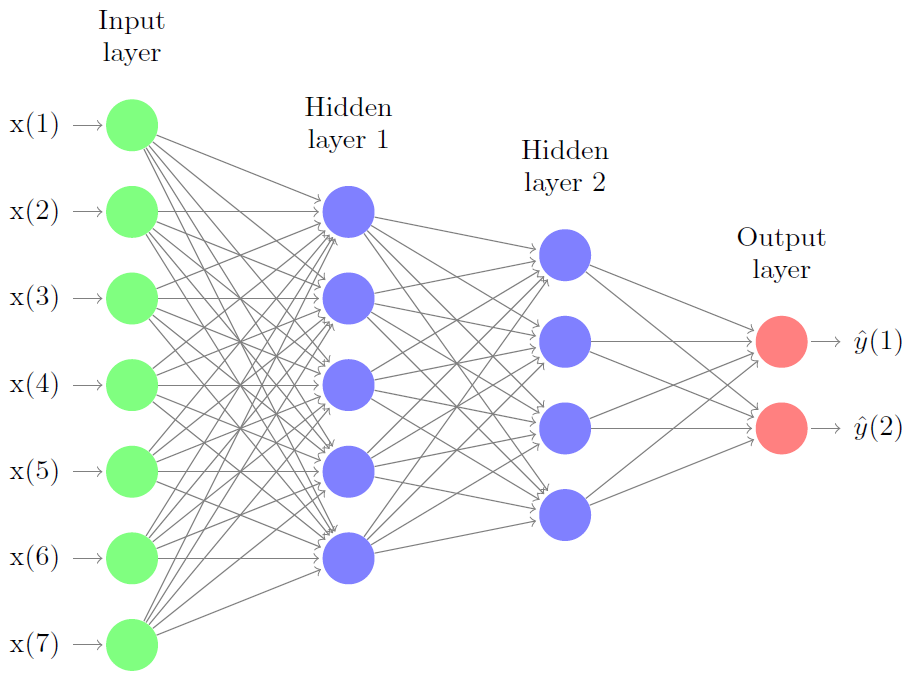
\includegraphics[width=150mm]{ann/deep_network_topology.png} }
    \caption{ 
        An illustrative example of a feed-forward
        neural network with two hidden layers, seven fea-
        tures and two output states. Deep learning networks
        typically have many more layers, use a large number
        of features and several output states or classes. The
        goal of learning is to find the weight on every edge
        that minimizes a loss function.
        }
    \label{fig:deep_network_topology}
\end{figure}

The input layer matches the feature space, so that there are
as many input neurons as predictors. The output layer is either a classification or regression 
layer to match the output space. All layers are composed of neurons, the basic units of such
a model. In the classical feedforward architecture, each neuron in the previous layer $ l $  is fully
connected with all neurons in the subsequent layer $ l + 1 $ via directed edges, each representing
a certain weight. Also, each neuron in a non-output layer of the net has a bias unit, serving
as its activation threshold. As such, each neuron $j$ of layer $l$ receives a weighted combination $ \alpha $ of the
$ n_{l - 1} $ outputs of the neurons $i = 1, ..., n_{l - 1} $ in the previous layer $ l - 1 $ as input,

\begin{equation}
    \alpha_{j}^{l} = \sum_{ i=1 }^{ n_{l - 1} } w_{i, j}^{l} x_{i}^{l - 1} + b_{j}^{l},
    \label{eq:dnn_alpha_weighted_combination}
\end{equation}

with $ w_{i, j}^{l} $ denoting the corresponding weight in layer $l$ for the input $ x_{i}^{l - 1} $ of the previous layer $l - 1$.
$ b_{j}^{l} $ denotes the bias for neuron $j$ of layer $l$. 
The weighted combination $ \alpha $ of equation \ref{eq:dnn_alpha_weighted_combination} is transformed via
some activation function $ f $, so that the output signal $ f(\alpha) $ is relayed to the neurons
in layer $ l + 1 $. Comparing equation \ref{eq:dnn_alpha_weighted_combination} and the Logistic Regression from chapter \ref{ch:logistic_regression}, 
the similarities become apparent. In that sense, a DNN can be interpretet as multiple sequences of Logistic Regression
chained together with different activation functions converging into the final model output.
We use the ReLU (rectified linear activation unit) (\cite{arora2018relu}, \cite{berner2019reluDerivative})
$ f: \mathbb{R} \rightarrow \mathbb{R} $,

\begin{equation}
    f( \alpha^{l} ) = max( \alpha^{l}, 0 ) = ( max\{0, \alpha^{l}_{1}\}, ..., max\{0, \alpha^{l}_{  n_{l}  }\} )^{T}
    \label{eq:relu}
\end{equation}

Let $ W $ be the collection $ W = \bigcup_{l=1}^{L - 1} W_{l} $, with $W_{l} = (w_{i, j}^{l}) \in \mathbb{R}^{ n_{l - 1} \times n_{l} } $ denoting the
weight matrix that connects layers $l$ and $l + 1$ for a network of L layers. Analogously, let $B$
be the collection $ B = \bigcup_{l=1}^{L - 1} b_{l}  $,
with $ b_{l} = ( b_{j}^{l} ) \in \mathbb{R}^{ n_{l - 1} } $ denoting the column vector of biases for layer $l$ such that the objective is to find
the optimal $ \theta = (W, B) $ parameters.
The collections $W$ and $B$ fully determine the output of the entire DNN. Learning is implemented
by adapting these weights in order to minimize the error on the training data. In particular,
the objective is to minimize some loss function $\mathscr{L} (\theta)$ for each training example $(x_{i}, y_{i}) \in D$. 
Since we are dealing with a classification problem, the loss function is cross-entropy,

\begin{equation}
    \mathscr{L} (\theta) = - \sum_{i=1}^{n} \sum_{ k=1 }^{K}  ln( m(y=y_{k} | x_{i}; \theta))  \cdot y_{k}
    \label{eq:dnn_loss_function}
\end{equation}

with $ m(y=y| x_{i}) $ denoting the fully parametrized DNN as a function according to $W$ and $B$ of feature vector $x_{i}$. 
Since we are using  the softmax function \cite{dixon2015annMarketPrediction} to transform the output from the last hidden layer,
the DNN can expressed as follows:

\begin{equation}
    m( y=y_{k} | x_{i} ) =  \frac{ \alpha_{c}^{L} }{ \sum_{j=1}^{K} \alpha_{c}^{L} }
\end{equation}

The loss function \ref{eq:dnn_loss_function} is minimized
by stochastic gradient descent, with the gradient of the loss function $\Delta_{\theta} \mathscr{L} (\theta)$
being calculated via backpropagation \cite{krauss2016arbitrageSandP}.
% More specifically, For each node $j$ in the $l - 1$-th layer, the recursion relation for the back
% propagation using conjugate gradients is \cite{dixon2015annMarketPrediction}:

% \begin{equation}
%     \delta_{j}^{l- 1} = \sum_{i=1}^{ n_{l} } \delta_{i}^{l}  w_{i, j}^{l} f^{'}( \alpha_{j}^{l-1} ),
%     \label{eq:back_propagation}
% \end{equation}

% with $f^{'}$ in our application being the derivative of the ReLU function defined as \cite{berner2019reluDerivative}

\begin{equation}
    f^{'}(\alpha^{l}) = ( \mathbb{I}(\alpha^{l}_{1} > 0), ..., \mathbb{I}(\alpha^{l}_{ n_{l} } > 0) )^{T}
\end{equation}

Following \cite{rojas1996neuralNetworks}, \cite{ruder2016gradientDescent}, and \cite{dixon2015annMarketPrediction},
the backpropagation learning algorithm based on the method of stochastic gradient descent (SGD) updates 
the parameters $ \theta $ after randomly drawing an observation $i$,

\begin{equation}
    \theta = \theta - \lambda \nabla_{ \theta } \mathscr{L}( \theta, i )
\end{equation}

with $\lambda$ denoting the learning rate.
Algorithm \ref{alg:stochastic_gradient_descent} below provides a high level description of the sequential version of
SGD.

\begin{algorithm}[H]
    \caption{ Stochastic Gradient Descent \cite{dixon2015annMarketPrediction} }

    \KwData{ Training set $D$ features and parameter space of DNN }

    \KwResult{ Optimized parameter values $\theta$ for DNN } 

    \tcc{ Draw initial parameter values from normal distribution }

    $ \theta \leftarrow r $ with $ r = (r_{i})_{i=1}^{n}  $ and $ r_{i} \in \mathscr{N}( \mu, \sigma ), \forall i $

    \tcc{ Get loss according to initial parametrisation }

    $ \mathscr{L} \leftarrow 0 $

    \For{ $  i \in \{ 1, ..., n \} $ }{
        $ \mathscr{L} \leftarrow \mathscr{L} + \mathscr{L}_{i}( \theta ) $
    }

    \tcc{ As long as loss above threshold $\tau$, continue to update $\theta$ }

    \While{ $ \mathscr{L} \geq \tau  $  }{

        \For{ $  i \in \{ 1, ..., n \} $ }{

            \tcc{ Draw random sample from data $D$ }

            $ i \leftarrow drawRamdomly(D) $

            $ \theta \leftarrow \theta - \lambda \nabla_{ \theta } \mathscr{L}( \theta, i ) $
        }

        $ \mathscr{L} \leftarrow 0 $

        \For{ $  i \in \{ 1, ..., n \} $ }{
            $ \mathscr{L} \leftarrow \mathscr{L} + \mathscr{L}_{i}( \theta ) $
        }
    }
    \label{alg:stochastic_gradient_descent}
\end{algorithm}


In order to describe the network's topology, we introduce the following notation: I-H1-H2-H3-H4-O.
I denotes the number of input neurons, H1, H2, H3 and H4 the number of hidden neurons in hidden layers 1, 2, 3, and O the number of output
neurons. A popular rule to set the number of neurons in the first hidden layer H1 of a feedforward network
is to use as many neurons as there are inputs \cite{krauss2016arbitrageSandP} which we also abide by.
To introduce a closer fit to the data, we also set H1 = H2.
Via the third and fourth hidden layer (H3 and H4), 
we introduce a bottleneck, enforcing a reduction in dimensionality in line with \cite{takeuchi2013momentumTrading} and 
\cite{dixon2015annMarketPrediction} resulting in H3 = 15 and H4 = 10.
Let $K$ be the number of features of the data. Then, our topology specification results in 
I-H1-H2-H3-O = $K$-$K$-$K$-15-10-2 with input layer I matching the number of features.
We train with 400 epochs, i.e., we pass 400 times over the training set, as in \cite{huck2009pairSelection}.
At this stage we would like to point that according to \cite{zhang1998annStateOfTheArt} the design of an ANN is more of an art than a science.
Therefore, we mainly followed best practices and intuitions to calibrate the DNN. 
However, for the purpose of this paper, it can be argued that it is sufficient, since it shows the operational costs aspect of such an endeavour.



\subsection{Trading Algorithm} \label{ch:trading_algorithm}
For trading phase, we proceed similarly to 
\cite{krauss2019statisticalArbitrage}, \cite{gatev2006pairsTrading} and \cite{krauss2016arbitrageSandP}.
After having trained each model for different specifications, we generate probability estimates for each class
based on the trading sets feature's. These probabilities for each bin are then used as signals in bin $t$ for each coin
in order for the algorithm to decide whether to enter or close a position invested in a coin in the next bin in $ t + 1 $.
We refer to these position as active.
More specifically, the algorithm compares the probability estimate for each coin and decides 
whether to close the current position and enter a new one. The coin with the highest probability estimate for a down movement
is considered as a candidate for the short position, if its probability is also above a certain threshold,
since it is most likely to go down. 
The algorithm proceeds analogously for the long position. 
If a coin gets chosen this way and the position for this movement is active, then it proceeds to close this position.
Therefore, we enter a long and a short position at most per bin $ t $.
In order get a better estimate of the return, we enter 60 initial short and long positions at different points in time,
thus the resulting portfolio has 120 active positions at most.
Then, we proceed to calculate aggregate values for each of these positions. To render the backtest more
realistic, we incorporate the following constraints:
\begin{basedescript}{%
    \desclabelstyle{\multilinelabel}
    \desclabelwidth{4,5cm}}
    \item[Minimum duration:] {
        Any active position has a minimum duration of $ d = 120, 240 $, before considering closing it.
    }
    \item[Execution gap:] {
        To account for the time it takes to generate a probability signal and submit the order accordingly,
        we introduce a execution gap of one minute. This means that when generating the signal from the bin in $ t $,
        the order gets executed in $ t + 1 $ the earliest.
    }
    \item[Minimum volume:] { 
        Orders for opening or closing a position only get executed in bin $ t $, 
        if any volume was traded in the respective bin.
    }
    \item[Order cancel:] {
        If after submitting the order in $ t $ the traded volume in bin $ t + 1 $
        is zero, the order gets canceled and a new probability signal gets generated in bin $ t + 1 $.
    }
    \item[Transaction cost:] {
        For every order execution a transaction cost of $ \epsilon $ bps gets subtracted. 
        Thus, the opening and closing of a position costs $ 2 \times \epsilon $ bps.
    }
    \item[Keep active position:] {
        If the probability signal yields the same coin as the one from the current active position,
        then keep the same position open for another $ d=120, 240 $ minutes before again generating another
        probability signal.
    }
\end{basedescript}


The algorithm described above can also be expressed in a pseudo-algorithmic way:

\begin{algorithm}[H]
    \caption{Pseudo-Algorithm for a single position ( short and long are analogous) }
    \KwData{ Minute-binned Test-OHLC-Data $OHLC$ and its estimated probabilities }
    \KwResult{ Trading decisions and its realized returns }

    Initiate \emph{Position}

    $row\_number \leftarrow 0 $

    \While{ $ row\_number < (max\_row\_number - delta) $ }{
        \tcc{ Load row data given by $ row\_number $ }

        $row \leftarrow OHLC.getRow( row\_number ) $

        \tcc{ Obtain maximum probability pair $max\_prob\_pair$ } 

        $max\_prob\_pair \leftarrow row.getMaxProbPair() $

        \tcc{ Determine whether probability condition is fulfilled }

        \uIf{ row.getProb( max\_prob\_pair ) $>$ threshold }{
            \uIf{ Position.active == False  }{
                Position.open()
            }
            \uElseIf{  max\_prob\_pair != Position.pair }{
                Position.close()
            }
        }
        \Else{
            \uIf{ Position.active == True }{
                Position.close()
            }
        }

        \tcc{ Skip minute bins based on current position }

        \uIf{ Position.active == True }{
            $ row\_number \gets row\_number + delta $
        }
        \Else{
            $ row\_number \gets row\_number + 1 $
        }
    }

    
   \end{algorithm}
   